%!TEX root = ../../../super_main.tex
\section{Collaboration with Group \emph{SW606F15}}
\label{sec:collaboration_with_group_sw606f15}

After a general GUI design meeting, a new sequence deletion method was suggested by the customers. Sequences are used in some of the applications that are being developed by the other GUI groups. Sequences are lists of pictograms that should be viewed in chronological order, when then represent a behavior/action sequence which the citizen can execute \parencite{birken_slides}. This could for example be the order in which a citizen should dress, e.g. taking off your old pants before putting on new pants as seen in \figref{fig:sequence_example}.

\begin{figure}[!htbp]
	\centering
	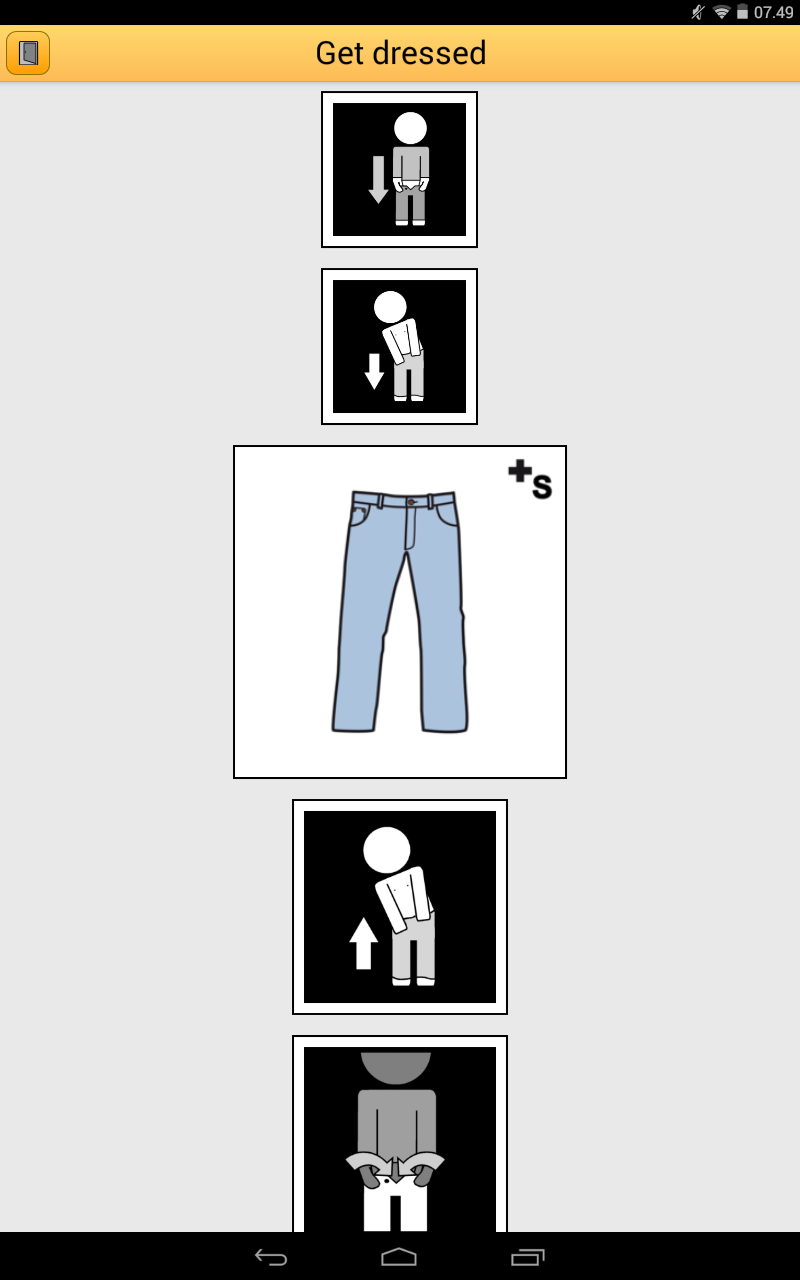
\includegraphics[width=0.5\textwidth]{sprint_three/sequence_example}
	\caption{Sequence viewer}
	\label{fig:sequence_example}
\end{figure}

\todo{Move the description of Sequence to possible appendix}

The application \emph{Sequence} manages a set of different sequences. It is required that different sequences can be removed. Previously when deleting sequences, the user would have to click a button to enter a ``Delete mode'' where, instead of clicking sequences to view them, clicks would delete the selected sequence. The customers requested the option to long-press a sequence to enter a ``Multi-selection mode'' where they were able to select multiple sequences in order to delete them. When a sequence is long pressed, the main menu is supposed to enter this mode and a trashcan button should appear in the top-bar \parencite{android_guidelines_longpress}. It should be possible to select and deselect sequences through regular press once inside the selection mode. It should furthermore be possible to deselect and exit the selection mode upon pressing the back button in the action bar. \todo{Det kunne være nice hvis man kom ud af den der selection mode hvis alt var unseleted (er det det?)}
\\\\
In our project, we had need for a feature like this one, which instead of selecting sequences was focused around selecting pictograms inside categories. To quickly overcome this task, we grouped up with \emph{SW606F15}, in order to resolve their issue first so we could implement the same structure in the two applications. The difference between the two projects is that our solution should select items using regular press, whereas theirs should initiate the selection with long-press followed by the actual selection using regular press.
\\\\
Previously, their project was based around the use of sequence objects and their respective identifiers to create views that represent the sequences. This resulted in not being able to find the view that belonged to the individual sequence, without passing both sequence and its view when using them in a method. This made it difficult to create the deselection feature when pressing the back button, since the back button was overriding the original \androidinline{onBackPressed} method, which does not take any parameters.
\\\\ 
Because of this we decided to implement a new data structure for their project which contains both a sequence and its respective view. This new structure made it possible to access the views that were selected and then deselect them when the back-button is pressed. 
\\\\
We furthermore implemented this using adapters as previously described, to improve performance when iterating through the list of sequences. This method of implementation could be directly transferred into our own project with minimal changes. An illustration of the final result can be seen in \figref{fig:sequence_multiselect}.

\begin{figure}[!htbp]
	\centering
	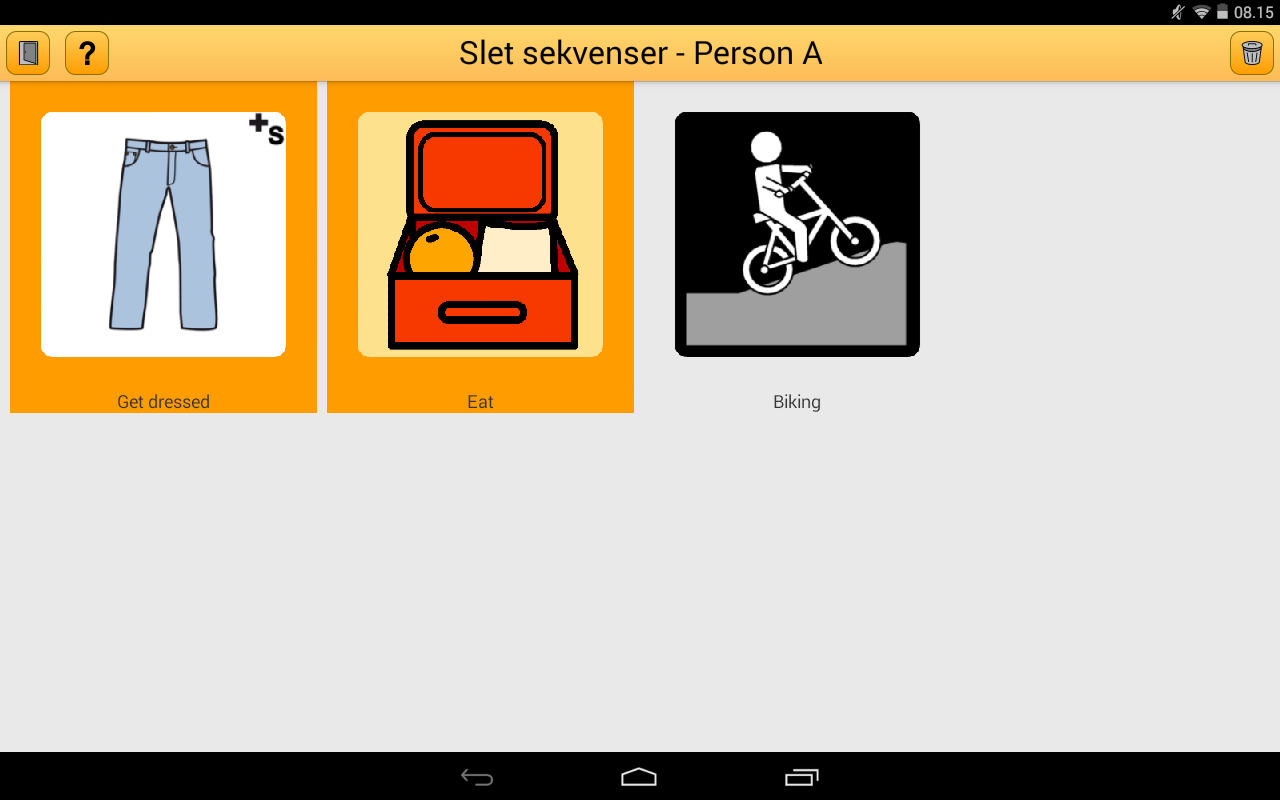
\includegraphics[width=\textwidth]{sprint_three/sequence_multiselect}
	\caption{Multiselect in sequence}
	\label{fig:sequence_multiselect}
\end{figure}